\section{XENONnT Detector}

% Brief intro to the XENONnT detector

XENONnT's sophisticated detector design generates complex, multidimensional signals that demand equally
sophisticated classification methods. This chapter details the detector systems and physics processes that
produce the \acrfull{s1} and \acrfull{s2} signals, establishing the technical context for understanding why traditional
classification methods proved insufficient and motivating our development of \acrfull{som}-based approaches.

The XENONnT experiment is located at the \acrfull{lngs} in Italy, beneath the Gran Sasso mountain. This underground location provides shielding from cosmic rays~\cite{PDG2024CosmicRays}, atmospheric muons, and radioactive isotopes present at the surface, such as $^{85}$Kr, which is released during the reprocessing of spent nuclear fuel whose global atmospheric abundance is estimated to be 5,500 PBq at the end of 2009 \cite{AHLSWEDE201334}. This deep underground location reduces background radiation in the detector, simplifies background modeling, and improves sensitivity to rare events such as WIMP-nucleon scattering. The low-background environment at \gls{lngs} has already enabled the first observation of double electron capture in the previous-generation XENON1T experiment~\cite{doubleEcapture}.

XENONnT is the most recent and sensitive detector in the XENON series of liquid xenon-based experiments, designed to search for dark matter interactions with baryonic matter. The experimental setup consists of three nested subsystems: a dual-phase liquid xenon \gls{tpc} at its core, surrounded by a gadolinium-loaded water Cherenkov neutron veto, which is itself enclosed by an external water Cherenkov muon veto (Fig. \ref{xenonnt_diagram_all_detectors}). The primary science goal is the detection of \glspl{wimp}, which are hypothesized to elastically scatter off xenon nuclei in the \gls{tpc}, producing measurable scintillation and ionization signals~\cite{PhysRevLett.131.041003}. However, this is only one of several key science channels explored by XENONnT. Recently, the experiment reported the first observation of $^8$B solar neutrinos with a xenon target, in parallel with the PandaX-4T collaboration~\cite{XENON:2024ijk, PhysRevLett.133.191001}. This chapter provides an overview of the experimental apparatus, the underlying detector physics, and the data processing pipeline.

\begin{figure}[htbp]
    \centering
    \includegraphics[origin=c, width=16cm]{figs/xenonnt_bkg/Xenonnt_diagram_mod.png}
    \caption{Figure showing the nested detectors of the XENONnT experiment. The outer layer is the muon veto, the neutron veto sits inside with the cryostat and the \gls{tpc} at the core.}
    \label{xenonnt_diagram_all_detectors}
\end{figure}


\subsection*{Muon veto}

The muon veto is a cylindrical water tank measuring $\SI{9.6}{m}$ in diameter and $\SI{10.2}{m}$ in height, filled with approximately 700\,tonnes of demineralized water.
It contains 84 \acrfull{pmt}s, each 8\,inches in diameter, arranged into five vertically spaced rings along the tank's perimeter. When muons traverse the water, they emit Cherenkov radiation, which is detected by the \glspl{pmt}. These signals allow us to tag muons and veto events occurring in temporal coincidence with their passage~\cite{XENON:2024wpa}.
There are three primary reasons for vetoing data in the vicinity of a muon signal. First, muons can induce secondary interactions that mimic \gls{wimp}-like signatures, thereby increasing the background and reducing the ability to distinguish signal from noise. Second, vetoing muon-related data improves the signal-to-noise ratio by removing events associated with high-energy cascades, often accompanied by intense Cherenkov emission~\cite{JVJelley_1955}. Lastly, background models are constructed under the assumption that muon-induced events and their secondary interactions are excluded, improving the robustness and accuracy of background predictions.  

\subsection*{Neutron veto}

The neutron veto plays a direct role in reducing background events that can mimic dark matter interactions. It contains 33\,m$^3$ of water doped with gadolinium sulfate with 120 8-inch PMTs. When thermalized neutrons are captured, they emit $\gamma$-rays that Compton scatter electrons, accelerating them to relativistic speeds. These electrons then emit Cherenkov radiation, which is detected by the \glspl{pmt}. Gadolinium was added to enhance neutron detection efficiency, as it has the highest thermal neutron capture cross section among all stable elements. Upon capturing a neutron, gadolinium emits a cascade of $\gamma$-rays totaling 7.9–$\SI{8.5}{MeV}$, which produce Cherenkov radiation via Compton scattering~\cite{Wenz2023thesis}. The neutron veto is also useful in calibrating our detector for \acrfull{nr}. We use an AmBe source for neutron calibration, where, 
$$^{241}Am \rightarrow ^{237}Np + \alpha, ^9Be + \alpha \rightarrow ^{12}C^* \text{(or }^{12}C) + n$$

The de-excitation of $^{12}\text{C}$ produces a $\SI{4.4}{MeV}$ $\gamma$-ray~\cite{ITO2023168701}. When the  $\gamma$-ray is emmited, it interacts with the surrounding medium, which generates $\gamma$-rays detectable by the \glspl{pmt}. We use these $\gamma$-rays to tag these neutrons resulting from the excited carbon for our \gls{nr} calibration. The time coincidence between signals in the neutron veto and \gls{tpc} enables tagging of neutron-induced nuclear recoils. This significantly reduces background from neutron events, which closely mimic \gls{wimp}-like signatures.

At the core of the veto systems lies the dual-phase liquid xenon \gls{tpc}. This is the primary detector volume for dark matter searches and will serve as the central focus of this work.

\subsection{Dual-phase Liquid Xenon TPC}


The TPC contains a \acrfull{lxe} target with a small gas gap of \acrfull{gxe} forming a dual-phase configuration. Throughout this work, the term ‘TPC’ will refer specifically to this detector volume. The detector contains 5.9\,tonnes of \gls{lxe} within a cylindrical volume 1.34\,m in diameter. It is housed in a double-walled, vacuum-insulated cryostat that maintains the xenon at a temperature of $-98\,^\circ$C.
Light is detected by two arrays of 3-inch Hamamatsu R11410-21 PMTs: 241 PMTs at the bottom and 253 at the top, for a total of 494. This configuration maximizes \acrfull{lce} given the geometry of the \gls{tpc}. Maximizing the \gls{lce} is a crucial part of our experiment as it ensures accurate energy reconstruction of the interactions within the \gls{tpc}. To enhance photon collection, the \gls{tpc} walls are lined with \acrfull{ptfe} panels due to their high reflectivity for xenon scintillation light at $\SI{175}{nm}$~\cite{FUJII2015293}, with estimates as high as 97$\%$ in some studies~\cite{Neves:2016tcw}. The exact reflectivity in XENONnT, however, remains uncertain.

Electrodes are used to generate electric fields within the \gls{tpc}, which are necessary to extract electrons released during particle interactions in the liquid xenon. This enables us to measure the energy deposited into the ionization process. The electric field is shaped and maintained by five parallel grid electrodes and two concentric cages of field-shaping rings. The parallel grid electrodes are configured as follows (from bottom to top):
\begin{itemize}
    \item A screening mesh located $\SI{5.3}{mm}$ above the bottom PMT array.
    \item A cathode located $\SI{60}{mm}$ above the first screening mesh.
    \item A gate electrode $\SI{5.02}{mm}$ below the liquid level/$\SI{1.486}{m}$ above the cathode.
    \item The anode $\SI{8}{mm}$ above the gate.
    \item A second screening electrode $\SI{40.7}{mm}$ below the top PMT array.
\end{itemize}
To mitigate electrode sagging due to electric field stress and gravity, two perpendicular support wires were added to the gate and four to the anode. A uniform drift field of approximately $\SI{20}{V/cm}$ is established between the cathode and gate, directing ionization electrons upward toward the liquid-gas interface. There, an extraction field between 2.9–$\SI{3.7}{kV/cm}$, applied between the gate and anode, pulls electrons into the gas phase~\cite{XENON:2024wpa}. The field shaping electrodes maintain a uniform electric field within the TPC, which maximizes the active volume.

\Glspl{pmt} are the photon-sensitive components of the detector, responsible for converting scintillation light into measurable electrical signals. 
%Discribe how PMTs work -> data read out to DAQ -> data processing
When photons reach the photoemissive cathode, they produce \acrfull{pe}. The \glspl{pe} are accelerated toward a series of dynodes by an internal electric field. At each dynode, they release secondary electrons, resulting in signal amplification. The amplified electron cascade is collected at the anode, producing a voltage pulse proportional to the energy deposited in the interaction~\cite{hamamatsuPMT}. The analog signals are digitized at $\SI{10}{ns}$ intervals and passed to the \acrfull{daq}, where they undergo initial processing and are stored on dedicated servers.



\begin{figure}[htbp]
    \centering
    \includegraphics[origin=c, width=16cm]{figs/xenonnt_bkg/PMT-schematics.png}    \caption{Depiction of how PMTs work. We see that the emitted photons react with the photoemissive cathode to produce photoelectrons, which are amplified by the dynodes and read out by the anode. The change in voltage is correlated with the number of incident photons \cite{pmt_fig}. }
    \label{pmt_schematics}
\end{figure}


\subsection{Why Xenon?}

A natural question in the context of dark matter detection is: why choose xenon as the target medium? There are many reasons to choose xenon for our detector, which are the following:
\begin{itemize}
    \item \textbf{Noble Gas}: chemically inert, ensuring minimal interactions with detector materials and reducing unpredictable background sources. This helps maintain a low and well-characterized background rate. 
    \item \textbf{Maximizing WIMP Nucleon Cross-section}: The spin-independent WIMP-nucleon cross-section scales approximately with the square of the atomic mass number ($A^2$). Therefore, a heavy nucleus like xenon enhances the detection probability for WIMPs.
    \item \textbf{Stable atomic nucleus}: While heavier noble gases like radon exist, they are radioactive. Xenon offers a balance of high atomic mass and isotopic stability, making it ideal for low-background experiments.
    \item \textbf{Xenon is well-suited for scintillation-based detection}: Xenon has a high photon yield, and it is transparent to its own emissions, ensuring that the full energy of the interaction can be captured by the PMTs. This occurs because excited xenon atoms form short-lived dimers (excimers), which de-excite by emitting vacuum ultraviolet (VUV) photons. Since xenon is transparent to its own scintillation light, the emitted photons can travel significant distances without being reabsorbed.
    \item \textbf{Xenon is self-shielding}: Due to its high density, xenon is effective at attenuating external radiation. This self-shielding property enables background reduction by selecting a fiducial volume away from the detector boundaries.
    \item \textbf{Xenon has a low electron affinity}: due to its properties as a noble gas, making it easy for electrons to travel within the TPC and reducing the chances of the electron being absorbed.
\end{itemize}

There are other direct detection experiments that use different atoms such as argon, to conduct the dark matter search. Argon offers superior discrimination between nuclear and \acrfull{er} via \acrfull{psd}, which exploits differences in scintillation time profiles between the two interaction types. It is crucial to distinguish nuclear recoils from electronic recoils as \glspl{wimp} are expected to interact primarily via coherent scattering off atomic nuclei, whereas most background events produce \glspl{er} \cite{Lippincott2008}. 

However, most of the leading limits are set using xenon as a medium due to its higher atomic mass, which enhances the spin-independent \gls{wimp}–nucleon cross-section and improves sensitivity to \gls{wimp} signals. Additionally, for \glspl{wimp} with masses near $\SI{100}{GeV}$, xenon offers favorable kinematic matching, maximizing energy transfer during elastic scattering.

\subsection{From Light Signals to Data}

With the detector structure described, we now turn to the atomic interactions responsible for signal generation. When a particle interacts with a xenon atom in the \gls{tpc} it will impart some energy onto it. This energy deposition may occur via an \gls{nr} or an \gls{er}, depending on whether the particle interacts with the xenon nucleus or its electrons. The deposited energy results in two measurable channels: excitation, which produces scintillation light, and ionization, which frees electrons from xenon atoms~\cite{Lanqing2025thesis}. \Glspl{er} typically produce more ionization electrons, while nuclear recoils result in a higher proportion of scintillation light due to increased recombination and excitation. In this process, the recoiling xenon atom or electron will form a short track in which it will excite or ionize other xenon atoms, which form dimers with other xenon atoms \cite{VChepel_2013}. Through excitation, the process is simple:

$$Xe^* +  Xe +  Xe\rightarrow Xe_2^* +  Xe + heat$$

In the case of ionization, some freed electrons may recombine with xenon ions, forming excimers and contributing to the scintillation signal. This process is known as recombination~\cite{VChepel_2013}. Although the ionization pathway involves additional steps, it ultimately results in the same xenon excimer responsible for scintillation light:

$$Xe^+ + Xe \rightarrow Xe_2^+$$
$$Xe_2^+ + e^- \rightarrow Xe^{**} + Xe$$
$$Xe^{**} + Xe \rightarrow Xe_2^* + \text{heat}$$

Here, $Xe^*$ and $Xe^{**}$ denote two excited states of xenon with are two excited states of xenon, with $Xe^{**}$ representing a higher energy state. These xenon dimers will decay on the scale of 10~ns, releasing vacuum ultraviolet (VUV) photons with a wavelength of \SI{175}{nm}.

$$Xe_2^* \rightarrow Xe + Xe + \gamma$$

This mechanism underlies the primary scintillation (S1) signal observed in xenon detectors. Two distinct scintillation signals are produced in a dual-phase xenon TPC:
\begin{itemize}
    \item the prompt scintillation signal (S1), generated immediately at the interaction site, and
    \item the delayed electroluminescence signal (S2), produced when ionization electrons are extracted into the gas phase and accelerated, causing secondary photon emission.
\end{itemize}

Free electrons drift to the top of the \gls{tpc} due to an electric field, and are then extracted into the gaseous xenon with a stronger extraction field. These electrons excite xenon atoms in the gas phase, forming excimers that subsequently de-excite and emit vacuum ultraviolet (VUV) photons—this is the basis of the S2 scintillation signal. Scintillation light produced in the detector is recorded by \glspl{pmt} located on the top and bottom arrays (Fig. \ref{pmt_schematics}). 

\begin{figure}[htbp]
    \centering
    \includegraphics[origin=c, width=16cm]{figs/xenonnt_diagram.jpg}
    \caption{Diagram of the XENONnT TPC illustrating the production of S1s and S2s in our detector. On the left, we see an incoming particle interacting with the liquid xenon, producing scintillation light detected by the top and bottom PMT arrays, which produces a response that is faster in time than the S2. On the right, we see the released electrons from the initial interaction pass the liquid/gas interface, generating scintillation light that is detected primarily by the top PMT array, which is more localized. This signal also results in a signal that is more spread out in time due to the difference in arrival time of the released electrons. }
    \label{xenonnt_diagram}
\end{figure}

In addition to true S1 and S2 signals, several spurious or non-physical signal types can occur in the \gls{tpc} and must be identified and removed during analysis. Gas-phase interactions: particles can interact directly with the gaseous xenon above the liquid surface, producing a prompt signal that mimics an S1 and induces a weak S2-like response. PMT afterpulsing occurs when residual gas atoms inside the \gls{pmt} vacuum become ionized and later strike the photocathode, producing delayed signals.
Dark counts refer to spurious signals caused by thermionic emission or electronic noise in the \gls{pmt} circuitry. In what follows, we focus on the primary S1 and S2 signals that form the foundation of event reconstruction.

\subsection{Background and Calibration Data.}

While data taking, the types of runs in the XENON experiment can be largely classified into two types, background and calibration data. Background data is used to conduct most analysis like the \gls{wimp} and $^8$B search and it involves running the experiment while minimizing all outside radiation sources. During calibration runs, we deliberately introduce a known source of radiation into our experiment, either by injecting it directly into the liquid xenon and removing it later, or by putting a radiation source in a mechanism that can be placed next to the \gls{tpc}. 

\begin{figure}
    \centering
    \includegraphics[origin=c, width=10cm]{figs/ted_bkg_fit_xenon.png}
    \caption{Background event rates in the XENONnT experiment as a function of \acrfull{ces}. Figure shows the different components associated with the background in our experiment and how they all contribute to our overall background rate.}
    \label{xenonnt_background}
\end{figure}

\subsubsection{Background data}

XENONnT is an experiment that requires the lowest background radiation possible. Because of this, there was significant investment in the mitigation of potential outside sources of radiation \cite{XENON:2021mrg}. Despite all these efforts, it is impossible to make this kind of experiment free from all sources of radiation.
The background radiation detected in XENONnT is primarily for electronic recoils, produced by $\beta$-decay from $^{214}$Pb and $^{85}$Kr. 

\subsubsection*{Radon222}

$^{222}$Rn particles are almost unavoidable as it is ubiquitous on the Earth's crust \cite{epa_radon_origin}. As a result, $^{222}$Rn will be part of the material components used to build the detector, making it an unavoidable radiation source which we need to take into account in our background models. $^{214}$Pb is a byproduct of the decay chain of $^{222}$Rn \cite{PhysRevD.111.103040}, and with its half-life of just 26.8\,mins, it and its subsequent daughter particles are a substantial contributor to our \gls{er} background and our $\alpha$ background. As these contaminants cannot be completely removed, our aim is to model this background accurately and subtract it from our main science channel searches.

\subsubsection*{Kr85}

Xenon is sourced from the atmosphere which contains other gasses that are not easily separable. We expect other impurities will be present, such as $^{85}$Kr, a byproduct of nuclear fission, introduced into the atmosphere via nuclear testing and nuclear reprocessing plants \cite{bollhoefer2020}. $^{85}$Kr decays to $^{85}$Rb via beta decay, which means it is also a source \gls{er} background over a continuous energy range. While $^{85}$Kr is an intrinsic impurity, we can still reduce its concentration via a cryogenic distillation column \cite{Guida:2025lif}.

\subsubsection*{Xenon Isotopes}

Even if we obtained a perfectly pure sample of xenon, it still would not free us of intrinsic backgrounds as unstable isotopes of xenon are also present in the atmosphere namely: $^{136}$Xe and $^{124}$Xe. While undesired for the main \gls{wimp} search channels, these backgrounds also allow us to explore new physics. $^{136}$Xe produces 2 $\beta$ particles, this is known as double $\beta$ decay \cite{double_beta_decay, PhysRevLett.59.2020}. According to theory, this could produce a rare interaction known as a neutrinoless double $\beta$ decay, which, if found, would show neutrinos are Majorana particles \cite{PhysRev.56.1184}. This is one of our current science search channels \cite{PhysRevC.106.024328}. On the other hand $^{124}$Xe was already the subject of a significant observation by the XENON collaboration as in XENON1T, we observed the first documented case of a double electron capture \cite{doubleEcapture}. As such, these are backgrounds that we do not attempt to remove from our experiment and must be taken into account in our background models.

\begin{figure}
    \centering
    \includegraphics[origin=c, width=14cm]{figs/Rn_decay_chain.png}
    \caption{Decay chains for Rn 222, a common source of background radiation in XENONnT and Radon 220 which is used as a calibration source. Figure credit \cite{Rn222_decay_chain}}
    \label{rn_decay}
\end{figure}

\subsubsection*{Neutrinos}

This is for all neutrinos, not just solar.
The sun produces neutrinos, which contribute to the background of our experiment; these are called solar neutrinos. These neutrinos can contribute to our background both via ER scattering and scattering off the nucleus of xenon atoms known as \acrfull{ceνns}. The signal produced by a CEνNS interaction is almost identical to a 6\,GeV/$c^2$ WIMP \cite{PhysRevLett.126.091301}. ER of neutrinos can be excluded from our analysis with relative ease however, NR recoils of neutrons is a major limitation of the WIMP search analysis.

\subsubsection*{Accidental Coincidences}

\acrfull{ac} are an artifact of our event reconstruction as they occur when we incorrectly pair an S1 and S2 signals. ACs can occur for a number of different reasons, including the misclassification of a single electron S2 signal as an S1. We refer to these S1/S2 signals that could be mismatched as ``isolated", as they lack a corresponding S2/S1 signal to match with. ACs happen when these signals occur within the event building time window \cite{PhysRevD.100.052014}. We calculate the background rate of ACs with a data-driven analysis and the formula: 
$$R_{AC} = R_{isoS1} \text{ x }R_{isoS2} \text{ x } \Delta t.$$

Where $R_{isoS1/S2}$ is the isolated S1/S2 rate and $\Delta t$ corresponds to the event building time window. To minimize the number of ACs in our analysis, we developed a gradient boosted decision tree classifier based on the S2 pulse shape and drift time to flag and exclude these signals \cite{PhysRevD.111.103040}.

\subsubsection*{Material Background}

% We dont we have to worry about the daughter products of Rn222 until lead
The XENON Collaboration built the XENONnT experiment using material screened for radiation to minimize background radiation from materials; however, obtaining materials with no radioactive impurities is almost impossible and extremely expensive. The \gls{tpc} walls are made of \gls{ptfe}, has been documented to absorb $^{222}$Rn \cite{Rn222_decay_chain}. This isotope of Rn is highly unstable and quickly decays to $^{210}$Pb. Following this decay chain we can expect two $\beta$ decays from $^{210}$Pb and $^{210}$Bi followed by the $\alpha$-decay of $^{210}$Po. Since we know the source of these events comes from the walls, we can heavily reduce this background by applying a fiducial volume cut whose boundaries we can determine by examining the monoenergetic $\alpha$ events from $^{210}$Po \cite{PhysRevD.111.103040}.

\subsubsection{Calibration data}

XENONnT has numerous radioactive isotopes it uses for detector calibration. In particular, calibration sources such as $^{83m}$Kr, $^{241}$AmBe, $^{220}$Rn and $^{37}$Ar are used to quantify the detector response to ionization radiation \cite{xenoncollaboration2024xenonntanalysissignalreconstruction}.  While we will not discuss all calibration sources here, we will go through the calibration sources relevant for this article.

\subsubsection*{Rn220}

$^{220}$Rn is used to calibrate the detectors' \gls{er} response. The decay chain of this atom provides a continuous \gls{er} spectrum at low energies thanks to its $\beta$ emitter daughter and is used to model our \gls{er} band \cite{Lang:2016zde, xenoncollaboration2024xenonntanalysissignalreconstruction}. Due to its shorter half-life of 55.8\,seconds, this isotope of Rn can be used for calibration as it quickly decays into $^{208}$Pb, which is not radioactive \cite{Murra:2022mlr}, making it safe to resume normal background runs shortly after.

\subsubsection*{Kr83m}

$^{83m}$Kr is a metastable version of Kr which decays producing 2 $\gamma$-rays of 32.1 and 9.4\,KeV with decay half-life of 1.83~hrs and 154~ns respectively \cite{Kastens:2009pa}. As with radon, $^{83m}$Kr can be injected directly into our detector and its slow first half-life gives enough time for a uniform distribution, making it useful for calibration of detector response as a function of spatial location. Furthermore, the mono-energetic decays can also be used as a sanity check to measure our ability to reconstruct the energies of these interactions.

\begin{figure}[htbp]
    \centering
    \includegraphics[origin=c, width=6cm]{figs/kr_decay_energies.pdf}
    \includegraphics[origin=c, width=9cm]{figs/kr83_decay.pdf}
    \caption{$^{83m}$Kr decay. Left: $^{83m}$Kr decay before becoming stable. Right: possible peaks we expect for the $^{83m}$Kr decay; bottom two plots show complications in the data, such as the merging of peaks that are close together in time. Figure credit: \cite{kr83_dacay}}
        \label{Kr_decay}
\end{figure}

\subsubsection*{AmBe}

$^{241}$AmBe is our neutron calibration source, which releases a neutron when Am decays and produces an $\alpha$ particle that is absorbed by the Be, which becomes carbon and emits a neutron. For a detailed description of this process, see \cite{Wenz2023thesis}. This calibration source produces neutrons in a continuous energy spectrum and, as such, can be used to model our \gls{nr} band. The source for this neutron emitter is located outside the \gls{tpc} cryostat, which means we can use the neutron veto to tag some of these events.

\subsubsection*{Ar37}

We use $^{37}$Ar for the calibration of low-energy interactions of \gls{dm}. $^{37}$Ar decays via electron capture and, depending on the electron shell the captured electron came from, produces different signals. If $^{37}$Ar captures an electron from the K-shell, it emits a 2.8224\,keV S1 signal and a corresponding ionization signal. If $^{37}$Ar captures an electron from the L-shell, it only produces an S1 signal of 0.2702\,keV. The photons released from this interaction are not energetic enough to ionize Xe; therefore, they do not produce S2 signals \cite{Boulton:2017hub}.

\subsection{Software Infrastructure}

To manage the complex chain of data processing, metadata tracking, and security, the XENON collaboration has developed a number of different packages to aid in our work. At the core of the data processing are \hyperlink{https://github.com/AxFoundation/strax}{Strax}, \hyperlink{https://github.com/XENONnT/straxen}{Straxen}, and \hyperlink{https://github.com/XENONnT/cutax}{Cutax}—-packages that handle waveform processing, XENON-specific extensions, and cut definitions, respectively. These packages operate through a plugin architecture, where each plugin is a class responsible for a specific step in the data processing chain. A configuration object called a context defines which plugins to use and manages the necessary metadata for each analysis which is handled by \hyperlink{https://github.com/XENONnT/xedocs}{Xedocs}. \hyperlink{https://github.com/XENONnT/utilix}{Utilix} is used for general configuration and provides access to the runs database, which stores metadata about processed data runs. A run refers to a continuous period of data acquisition, typically characterized by its duration and data type (e.g., calibration, background, science), and is referenced by its unique run\_ids. We will discuss the software infrastructure in more detail in Sec. \ref{sec: Software_Infrastructure}.


\begin{comment}
data processing and other day to day organizational infrastructure the XENON collaboration has developed a number of different softwares with different applications. 
\begin{itemize}
    \item \hyperlink{https://github.com/AxFoundation/strax}{Strax}: an analysis framework for pulse-only digitization data. It is mainly build to support noble liquid TPC experiments such as XENONnT.
    \item \hyperlink{https://github.com/XENONnT/utilix}{Utilix}: utility package serving 2 main functions: (1) a general xenon configuration framework and (2) grants access to our runs database.
    \item \hyperlink{https://github.com/XENONnT/xedocs}{Xedocs}: Used for reading and writing to our metadata dataabse, which include corrections used for data processing.
    \item \hyperlink{https://github.com/XENONnT/straxen}{Straxen}: Main software for data analysis of the XENONnT collaboration, built on top of strax and integrates utilix and xedocs. Converts data from raw PMT readouts to energy meassurments of the intractions.
    \item \hyperlink{https://github.com/XENONnT/cutax}{Cutax} Software build on straxen, used to manage cuts for data cleaning necessary for data analysis.
\end{itemize}
We will expand on the software infrastructure in a later chapter.
\end{comment}

\subsection{Data corrections}

To accurately reconstruct particle interactions in the detector, we apply corrections at multiple stages throughout the data processing pipeline. These include corrections for converting PMT voltage traces to photoelectrons (during record formation) and accounting for the electron drift velocity to reconstruct the interaction depth. We use xedocs to manage the metadata associated with each correction, while enforcing rules and constraints to preserve data integrity during schema updates.
Some of these corrections or schemas, as we will call them henceforth, need different rules.


One key correction is the electron lifetime correction. As electrons drift through the liquid xenon, some are absorbed by electronegative impurities, reducing the number that reach the gas phase and contribute to the S2 signal. The electron lifetime characterizes this absorption and is used to correct the S2 area by extrapolating it to what would have been observed with infinite purity. Since electron lifetime changes over time, it must be carefully tracked and applied per-run. This is one of many time- and position-dependent corrections, making robust metadata handling essential—precisely the role of xedocs.

The metadata corrections tend to vary the most between different \acrfull{sr}. Science runs are designated time periods in which we collect data with the aim of publishing a result, usually to release our WIMP analysis. As of writing, XENONnT has had 3 science runs: SR0, SR1, and SR2. SR0 occurred shortly after the end of the commissioning phase of our detector and was used for our first set of results. After we were done with the analysis for SR0, we decided to make significant changes to the configuration of the detector for SR1. Major changes in the detector usually occur between science runs. For our purposes, we will only focus on the changes between science runs that affect low-level data. Between SR0 and SR1, there were significant changes to the way we adjust the PMT gains, affecting the characteristics of the waveforms generated. For our purposes, there is no difference between SR1 and SR2.


\subsection{Achievements of the XENONnT Experiment}

\subsubsection{WIMP constrain}

In February 2025, XENONnT released its latest results from the search for WIMP elastic scattering on xenon nuclei, combining the results of their two science runs (SR0 + SR1). The datasets consisted of 186.5 (95.1)\,days of livetime in SR1 (SR0) for a total exposure of $\SI{3.1}{tonne\cdot year}$. No significant excess above background was observed for nuclear recoil energies above $\SI{3.8}{keV_{nr}}$. We set a new upper limit in the spin-independent WIMP-nucleon scattering cross section for WIMPs of masses above 10\,GeV/c$^2$. The lowest cross-section limit reached was $1.7 \times 10^{-47}$\,cm$^2$ at 90\% confidence level for a WIMP mass of 30\,GeV/c$^2$. The best median sensitivity achieved was $1.4 \times 10^{-47}$\,cm$^2$ for a 41\,GeV/c$^2$ WIMP \cite{XENON:2025vwd}. Although we did not achieve a lower limit than LZ with our current data, the validation of the dark matter exclusion cross section is still an important check (Fig. \ref{wimp_results}).

\begin{figure}[htbp]
    \centering
    \includegraphics[origin=c, width=12cm]{figs/xenonnt_bkg/wimp_nucleon_cross_section_2024.png}    \caption{WIMP-nucleon cross section limits as a function of WIMP mass for the leading direct detection dark matter experiments. We see that while we obtained a lower limit than PandaX-4t the leading sensitivity, are places by LZ in this channel \cite{XENON:2025vwd}.}
    \label{wimp_results}
\end{figure}

\subsubsection{Detection of Solar neutrinos}

In November 2024, the XENON collaboration published a paper detailing the first measurement of nuclear recoils from $^8$B solar neutrinos via CEνNS. We conducted a blind analysis with an exposure of {3.51}\,{tonne$\cdot$yr} resulting in 37 observed events above 0.5\,keV compared to a background expectation of $26.4^{+1.4}_{-1.3}$ events. This corresponds to a rejection of the background-only hypothesis with a significance of 2.73$\sigma$ \cite{XENON:2024ijk}. The measured $^8B$ solar neutrino flux is consistent with the observations at the Sudbury Neutrino Observatory \cite{SNO:2011hxd}. We also report that the measured neutrino cross section on Xe is consistent with the Standard Model predictions. This marks the first direct detection of nuclear recoils from solar neutrinos using a dark matter detector \cite{XENON:2024ijk}.

\begin{figure}[htbp]
    \centering
    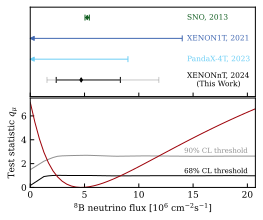
\includegraphics[origin=c, width=12cm]{figs/xenonnt_bkg/b8_unblinding_1d_cl_68.png}    \caption{$^8B$ neutrino flux for different experiments. We see that the tighter limits were set by SNO in 2013 \cite{SNO:2011hxd} with a dedicated neutrino experiment. In the latest XENONnT results, we obtained a tighter constraint from other direct detection dark matter experiments, results which are consistent with SNO.}
    \label{b8_results}
\end{figure}

\subsection{Scope}

In this document, we primarily focus on two dark matter detectors. These are the XENONnT detector, designed to detect dark matter and other rare interactions, and the XAMS experiment, which aims to test emerging TPC technologies.

Both experiments operate under the same physical principles and share a similar software architecture for data analysis. The differences between the two will be discussed when needed but we focus primarily on XENONnT, as the Nikhef-based XAMS detector serves as a simplified test platform for its technologies. This section emphasizes XENONnT, with a more detailed discussion of XAMS provided in later chapters.

\newpage